\documentclass[11pt,a4paper]{article}

% ====================== PACKAGES ======================
\usepackage[a4paper, top=2.4cm, bottom=2.4cm, left=2.2cm, right=2.2cm, headheight=16pt, headsep=14pt]{geometry}
\usepackage[T1]{fontenc}
\usepackage[utf8]{inputenc}
\usepackage{lmodern}
\usepackage{microtype}
\usepackage[table]{xcolor}
\usepackage{colortbl}
\usepackage{graphicx}
\usepackage{tabularx}
\usepackage{booktabs}
\usepackage{array}
\usepackage{titlesec}
\usepackage{enumitem}
\usepackage{tcolorbox}
\usepackage{fancyhdr}
\usepackage{longtable}
\usepackage{caption}
\usepackage{float}
\usepackage{pdflscape}
\usepackage[backend=biber,style=ieee,sorting=none]{biblatex}
\usepackage{hyperref}

% ====================== COLOR THEME (BLUE) ======================
\definecolor{tr1Blue}{HTML}{0D47A1}
\definecolor{tr1BlueMid}{HTML}{1565C0}
\definecolor{tr1BlueLight}{HTML}{1976D2}
\definecolor{tr1BlueSky}{HTML}{42A5F5}
\definecolor{tr1BlueBg}{HTML}{E3F2FD}
\definecolor{tr1BlueRow}{HTML}{F4F9FE}
\definecolor{tr1BlueDeep}{HTML}{082F66}

% ====================== HYPERREF (CLICKABLE TOC) ======================
\hypersetup{
  colorlinks=true,
  linkcolor=tr1Blue,
  filecolor=tr1Blue,
  urlcolor=tr1BlueLight,
  citecolor=tr1BlueLight,
  pdftitle={TR1NITY Phase 1 Report — Network Security},
  pdfauthor={Hamza, Irtaza, Hammad},
  pdfsubject={Unified SIEM Correlation Platform},
  pdfkeywords={Wazuh, Firewall, WAF, SIEM, Correlation, Foundation-Sec-8B, SIGMA, MITRE ATT&CK},
  pdfborder={0 0 0},
  bookmarks=true,
  bookmarksnumbered=true,
  bookmarksopen=true,
  pdfstartview={FitH}
}

% ====================== HEADERS / FOOTERS ======================
\pagestyle{fancy}
\fancyhf{}
\renewcommand{\headrulewidth}{0.4pt}
\renewcommand{\headrule}{\hbox to\headwidth{\color{tr1Blue}\leaders\hrule height \headrulewidth\hfill}}
\renewcommand{\footrulewidth}{0pt}
\fancyhead[L]{\textcolor{tr1Blue}{\small\textbf{AU} \,|\, Network Security}}
\fancyhead[R]{\textcolor{tr1Blue}{\small\textit{TR1NITY — Phase 1 Report}}}
\fancyfoot[C]{\textcolor{tr1Blue}{\small Dept. of Cyber Security \,|\, Air University Islamabad — Page \thepage}}

% Make 'plain' page style (used by TOC, chapter pages, etc.) match the fancy style
\fancypagestyle{plain}{
  \fancyhf{}
  \renewcommand{\headrulewidth}{0.4pt}
  \renewcommand{\headrule}{\hbox to\headwidth{\color{tr1Blue}\leaders\hrule height \headrulewidth\hfill}}
  \fancyhead[L]{\textcolor{tr1Blue}{\small\textbf{AU} \,|\, Network Security}}
  \fancyhead[R]{\textcolor{tr1Blue}{\small\textit{TR1NITY — Phase 1 Report}}}
  \fancyfoot[C]{\textcolor{tr1Blue}{\small Dept. of Cyber Security \,|\, Air University Islamabad — Page \thepage}}
}

% ====================== SECTION FORMATTING ======================
\renewcommand{\thesection}{\arabic{section}.}
\renewcommand{\thesubsection}{\arabic{section}.\arabic{subsection}}
\renewcommand{\thesubsubsection}{\arabic{section}.\arabic{subsection}.\arabic{subsubsection}}
\titleformat{\section}
  {\color{tr1Blue}\Large\bfseries}
  {\thesection}{0.6em}{}
\titleformat{\subsection}
  {\color{tr1BlueMid}\large\bfseries}
  {\thesubsection}{0.6em}{}
\titleformat{\subsubsection}
  {\color{tr1BlueLight}\normalsize\bfseries}
  {\thesubsubsection}{0.6em}{}

\titlespacing*{\section}{0pt}{14pt}{8pt}
\titlespacing*{\subsection}{0pt}{10pt}{4pt}

% ====================== TOC FORMATTING ======================
\usepackage{tocloft}
\renewcommand{\contentsname}{\textcolor{tr1Blue}{Contents}}
\setlength{\cftsecnumwidth}{2.6em}
\setlength{\cftsubsecnumwidth}{3.0em}
\renewcommand{\cftsecfont}{\color{tr1Blue}\bfseries}
\renewcommand{\cftsecpagefont}{\color{tr1Blue}\bfseries}
\renewcommand{\cftsubsecfont}{\color{tr1BlueMid}}
\renewcommand{\cftsubsecpagefont}{\color{tr1BlueMid}}
\renewcommand{\cftdotsep}{1.5}

% ====================== CAPTIONS ======================
\captionsetup[figure]{labelfont={color=tr1Blue,bf}, textfont={color=tr1Blue}, labelsep=period, font=small}
\captionsetup[table]{labelfont={color=tr1Blue,bf}, textfont={color=tr1Blue}, labelsep=period, font=small}

% ====================== TABLES ======================
\renewcommand{\arraystretch}{1.25}
\arrayrulecolor{tr1Blue}

\newcolumntype{L}[1]{>{\raggedright\arraybackslash}p{#1}}

% ====================== CALLOUT BOXES ======================
\newtcolorbox{problembox}{
  colback=tr1BlueBg,
  colframe=tr1Blue,
  boxrule=0.7pt,
  arc=2.5pt,
  left=8pt, right=8pt, top=6pt, bottom=6pt,
  fontupper=\color{tr1BlueDeep}\itshape
}

\newtcolorbox{infobox}[1]{
  colback=tr1BlueBg,
  colframe=tr1BlueMid,
  boxrule=0.6pt,
  arc=2pt,
  left=8pt, right=8pt, top=4pt, bottom=4pt,
  title={\color{white}\bfseries #1},
  coltitle=white,
  colbacktitle=tr1BlueMid,
  fonttitle=\bfseries
}

% ====================== BIBLIOGRAPHY ======================
\addbibresource{references.bib}

% ====================== DOCUMENT ======================
\begin{document}

% ============== COVER PAGE ==============
\begin{titlepage}
\thispagestyle{empty}
\noindent\hspace*{-0.5cm}\colorbox{tr1Blue}{\parbox{\dimexpr\textwidth+1cm}{%
  \vspace{12pt}
  \centering
  {\color{white}\Large\bfseries AIR UNIVERSITY, ISLAMABAD}\\[3pt]
  {\color{white}\large Department of Cyber Security}\\
  \vspace{12pt}
}}

\vspace{2.0cm}

\begin{center}
{\color{tr1BlueMid}\Large\bfseries NETWORK SECURITY}\\[6pt]
{\color{tr1BlueMid}\Large\bfseries PHASE-1 PROJECT DOCUMENTATION}

\vspace{1.6cm}

{\color{tr1Blue}\fontsize{42pt}{48pt}\selectfont\bfseries TR1NITY}

\vspace{0.8cm}

{\color{tr1BlueMid}\large\itshape Unified SIEM Correlation Platform for Wazuh, \\[2pt] Firewall, and WAF Logs}

\vspace{0.4cm}

{\color{tr1BlueLight}\normalsize ``Three sources. One brain. One cockpit. Zero license cost.''}

\vspace{1.6cm}

\noindent\colorbox{tr1BlueBg}{\parbox{0.85\textwidth}{%
\vspace{4pt}
\begin{flushleft}
\color{tr1Blue}
\textbf{Group Member Name:} Hamza\\
\textbf{Group Member Name:} Irtaza\\
\textbf{Group Member Name:} Hammad\\[6pt]
\textbf{Course:} Network Security\\
\textbf{Semester:} Spring 2026\\
\textbf{Submission Date:} \today\\
\textbf{Phase:} Phase 1 — Project Documentation
\end{flushleft}
\vspace{4pt}
}}

\vfill

\noindent\colorbox{tr1BlueDeep}{\parbox{\dimexpr\textwidth-2pt}{%
\vspace{6pt}
\centering
{\color{white}\small\itshape This project is designed for defensive security purposes only. All tools and integrations are used strictly within authorized and controlled environments.}\\
\vspace{6pt}
}}

\vspace{0.6cm}
\end{center}
\end{titlepage}

% ============== ABSTRACT ==============
\section{Abstract}
\label{sec:abstract}

Modern Security Operations Centers (SOCs) are saturated with disconnected log sources: Host-based Intrusion Detection Systems (Wazuh), perimeter and host firewalls (iptables, pfSense, OPNsense), Web Application Firewalls (ModSecurity / OWASP CRS), and optionally network IDS sensors (Suricata). Each source produces alerts in a different schema with different semantics. Analysts pivot constantly between dashboards, manually stitch evidence across sources, and lose critical response time under alert overload. Industry research consistently identifies alert fatigue as the single largest driver of analyst burnout, affecting an estimated 71\% of SOC analysts \cite{secure2024burnout}, and as the dominant factor behind 80\% of analyst time being consumed by low-fidelity alert clearance \cite{vmware2020soc}.

\textbf{TR1NITY} addresses this challenge with a unified, fully open-source, AI-assisted correlation platform that ingests Wazuh alerts, firewall logs, and WAF logs into a single normalized index, applies temporal correlation, entity resolution, MITRE ATT\&CK tagging, threat-intelligence enrichment, and a three-layer false-positive reduction pipeline. The platform exposes the result through a purpose-built React analyst workstation that consolidates the investigation workflow into a single-pane cockpit. A locally-hosted, security-specialized large language model (Foundation-Sec-8B \cite{cisco2025foundationsec}) drafts post-incident reports, runbooks, and compliance documents asynchronously, in line with empirical evidence that AI in SOCs is most beneficial for asynchronous writing tasks rather than real-time triage decisions \cite{darrow2024aisoc}.

The Phase-1 contribution is a complete architecture and implementation blueprint covering six modules: (1) Multi-source Ingestion \& Normalization, (2) Correlation \& Threat Intelligence (``The Brain''), (3) AI Assist (asynchronous, human-in-the-loop), (4) False-Positive Handling, (5) Analyst Workstation (``The Cockpit''), and (6) Knowledge \& Reporting. The platform is designed to run on commodity hardware (16~GB RAM, AMD RX 590 8~GB VRAM via the \texttt{llama.cpp} Vulkan backend), uses no paid APIs, and is deployable via a single Docker Compose command. Expected outcomes include a 70\%+ reduction in time-to-triage, a measured false-positive rate below 30\% within two weeks of analyst feedback, and full ATT\&CK Enterprise coverage visualization. TR1NITY is positioned as the first open-source platform to unify Wazuh, firewall, and WAF log streams under one correlation engine with an integrated analyst-first UI and a fully local LLM assistance layer.

% ============== TABLE OF CONTENTS ==============
\newpage
\thispagestyle{fancy}
\section*{\textcolor{tr1Blue}{\Large 2.\quad Table of Contents}}
\addcontentsline{toc}{section}{2.\quad Table of Contents}
\label{sec:toc}
\renewcommand{\contentsname}{}
\vspace{0.3cm}
\begingroup
\let\clearpage\relax
\tableofcontents
\endgroup
% Reset section counter so the next section becomes 3
\setcounter{section}{2}

% ============== INTRODUCTION ==============
\newpage
\section{Introduction}
\label{sec:introduction}

\subsection{Background}
Security operations have evolved from perimeter-only defense into a layered, telemetry-driven discipline that depends on host agents, network sensors, application-layer filters, identity systems, and external threat intelligence. As organizations adopted best-of-breed tools over the past decade, defensive depth improved dramatically while operational coherence eroded. Most SOCs now run separate consoles for endpoint detection, network detection, web application filtering, log aggregation, threat-intel enrichment, case management, and incident reporting — each with distinct schemas and alert semantics \cite{sans2024survey}. The consequence is that analysts perform extensive cognitive normalization manually: copying an IP from one tool, pasting it into another, mentally cross-referencing timestamps, and reconstructing kill-chains across windows.

This fragmentation is most acute at the intersection of three commonly-deployed open-source defenses: \textbf{Wazuh} (host-based IDS, file integrity monitoring, log forwarding), \textbf{firewalls} (iptables, pfSense, OPNsense), and \textbf{WAFs} (ModSecurity with the OWASP CRS). Each produces high-fidelity events for its own perspective, but no widely-adopted open-source platform unifies all three under one correlation engine with an analyst-first UI.

\subsection{Importance of the Domain}
Adversaries increasingly chain reconnaissance, credential abuse, web exploitation, and lateral movement at machine speed. A single intrusion campaign typically generates events across all three of TR1NITY's source classes — for example, an external port scan (Suricata / firewall), a SQL injection attempt (WAF), and a subsequent file-integrity violation on the compromised host (Wazuh). Without unified correlation, these events appear as three independent ``incidents'' across three tools, multiplying analyst workload and inflating mean-time-to-respond (MTTR). Industry data continues to show that the median MTTR for such cross-domain incidents in fragmented SOCs exceeds 200 hours \cite{ibm2024xforce}.

AI-assisted SOC tooling is now a strategic priority, but its empirical track record is nuanced. Real analysts report that current AI tools are most useful for asynchronous tasks (report drafting, runbook starters, summary generation) and \emph{least} useful for autonomous real-time triage decisions, where hallucinations and confident-but-wrong correlations measurably degrade analyst quality \cite{darrow2024aisoc}. This evidence directly shapes TR1NITY's AI design: the LLM \emph{drafts}, the human \emph{decides}.

\subsection{Problem Statement}
\begin{problembox}
Open-source SOC stacks force analysts to manually correlate Wazuh, firewall, and WAF events across three separate dashboards. False-positive rates of community detection content commonly exceed 60\% before tuning. No widely-adopted open-source platform combines a unified ingestion layer for these three log streams, a multi-layer false-positive reduction pipeline, an analyst-first single-pane investigation UI, and a fully local AI assistant for asynchronous report drafting — all without paid APIs and deployable on commodity hardware.
\end{problembox}

\subsection{Proposed Solution}
TR1NITY is structured as a six-module layered architecture, each module attacking a documented analyst pain point:

\begin{enumerate}[leftmargin=*, itemsep=2pt]
  \item \textbf{Module 1 — Ingestion \& Normalization:} Wazuh manager + Filebeat + a Python ingestor service consume webhooks and syslog from Wazuh, iptables/pfSense, and ModSecurity, mapping every event to a unified Elastic Common Schema (ECS) JSON document and writing to a single OpenSearch index \texttt{tr1nity-events-*}.
  \item \textbf{Module 2 — Correlation \& Enrichment (``The Brain''):} A FastAPI \texttt{correlator} service performs temporal grouping, entity resolution, MITRE ATT\&CK tagging, free threat-intel enrichment (AbuseIPDB, AlienVault OTX, NVD, abuse.ch), SigmaHQ rule import and translation via \texttt{pySigma}, and runbook auto-attachment.
  \item \textbf{Module 3 — AI Assist (HITL):} A local Foundation-Sec-8B-Instruct model running at Q4\_K\_M quantization (\textasciitilde{}5\,GB) via \texttt{llama.cpp} with the Vulkan backend on the AMD RX 590. Drafts post-incident reports, runbooks, and compliance documents. Never autonomously decides on alerts.
  \item \textbf{Module 4 — False Positive Handling:} A three-layer pipeline: (a) deterministic YAML whitelists, (b) a \texttt{scikit-learn} classifier trained on analyst feedback, and (c) analyst-authored suppression rules.
  \item \textbf{Module 5 — Analyst Workstation (``The Cockpit''):} React + TailwindCSS + shadcn/ui SPA delivering an alert queue, single-pane investigation panel (raw payload + enrichment sidebar + entity timeline + similar-incidents semantic search), MITRE ATT\&CK Navigator heatmap, and a lightweight built-in case manager.
  \item \textbf{Module 6 — Knowledge, Audit \& Reporting:} 15+ runbooks rendered to UI, full analyst audit trail in PostgreSQL, compliance PDF generator (PCI-DSS, ISO 27001, NIST CSF), weekly metrics report, and a one-command backup/restore.
\end{enumerate}

% ============== LITERATURE REVIEW ==============
\newpage
\section{Literature Review}
\label{sec:litreview}

Prior research and industry analysis converge on a consistent diagnosis: SOC inefficiency is dominated by alert fatigue, fragmented tooling, and poor automation pay-off when the underlying schema is non-uniform. Studies repeatedly link alert fatigue to workload saturation and low signal-to-noise ratios in enterprise monitoring \cite{secure2024burnout, vmware2020soc, sans2024survey}. SIEM-centric architectures improve event retention and compliance posture but rarely deliver end-to-end response automation or cross-platform reasoning \cite{nasr2022siem}. Machine-learning approaches have produced measurable gains in alert prioritization and intrusion detection on benchmark datasets such as CICIDS2017 and UNSW-NB15 \cite{sharma2023ml, martinez2021dl}, though production deployments routinely struggle with model drift and dataset realism. Suricata and Snort remain the canonical open-source NIDS engines but require ongoing rule-tuning effort to maintain acceptable false-positive rates \cite{almansoori2024nids}.

Threat-intelligence platforms such as MISP and OpenCTI have improved indicator sharing and enrichment fidelity, yet integration maturity across heterogeneous SOC stacks varies widely \cite{wagner2022ti}. SOAR adoption studies show meaningful reductions in repetitive analyst toil, balanced by playbook-governance and maintenance overhead \cite{collier2023soar}. Wazuh-focused academic work demonstrates strong open-source endpoint visibility for cost-constrained organizations \cite{qureshi2024wazuh}. Recent studies on LLM-assisted analyst workflows report time savings on summarization and drafting tasks, alongside the well-documented hallucination risk that necessitates human-in-the-loop guardrails \cite{nguyen2025llm, darrow2024aisoc}. Finally, the release of Foundation-Sec-8B \cite{cisco2025foundationsec} as a security-specialized open-weight LLM materially changes the cost-benefit balance for locally-hosted SOC AI assistance.

\subsection{Comparative Analysis of Prior Work}

\begin{table}[H]
\small
\setlength{\tabcolsep}{4pt}
\begin{tabularx}{\textwidth}{|>{\columncolor{tr1BlueBg}}L{2.4cm}|L{2.5cm}|L{2.0cm}|L{2.0cm}|L{2.0cm}|L{2.0cm}|}
\hline
\rowcolor{tr1Blue}\textcolor{white}{\textbf{Author / Year}} & \textcolor{white}{\textbf{Method / Approach}} & \textcolor{white}{\textbf{Tools Used}} & \textcolor{white}{\textbf{Dataset}} & \textcolor{white}{\textbf{Pros}} & \textcolor{white}{\textbf{Cons}} \\
\hline
S. Kent et al. (2021) \cite{kent2021soc} & SOC workflow study on analyst load & SIEM + ticketing & Enterprise SOC logs & Real-world fatigue evidence & No technical unification model \\
\hline
M. Nasr et al. (2022) \cite{nasr2022siem} & SIEM performance and triage delay analysis & Splunk, ELK & Synthetic + enterprise mix & Scalable ingestion insights & Limited response automation \\
\hline
R. Sharma et al. (2023) \cite{sharma2023ml} & ML classifier for alert prioritization & Python, XGBoost & CICIDS2017 & Better prioritization accuracy & Model drift risk \\
\hline
A. Martinez et al. (2021) \cite{martinez2021dl} & Deep IDS for hybrid networks & Suricata + LSTM & UNSW-NB15 & Strong detection recall & High training cost \\
\hline
K. Al-Mansoori (2024) \cite{almansoori2024nids} & Signature/rule tuning in NIDS & Snort, Suricata & DARPA + lab traces & Practical rule hardening & High FP-tuning effort \\
\hline
F. Wagner et al. (2022) \cite{wagner2022ti} & Threat-intel correlation in SOCs & MISP, OpenCTI & Public IOC feeds & Better IOC context depth & Feed quality variance \\
\hline
J. Collier et al. (2023) \cite{collier2023soar} & SOAR playbook automation impact & Shuffle, Cortex XSOAR & SOC incident records & Faster containment cycles & Playbook maintenance overhead \\
\hline
H. Qureshi et al. (2024) \cite{qureshi2024wazuh} & Endpoint telemetry correlation & Wazuh, Elastic & University SOC data & Open-source practicality & Endpoint-only blind spots \\
\hline
L. Nguyen et al. (2025) \cite{nguyen2025llm} & AI-assisted log summarization & ELK + LLM API & Mixed production logs & Analyst time reduction & Prompt governance needed \\
\hline
A. Darrow et al. (2025) \cite{darrow2024aisoc} & Empirical study of AI in MSSP SOCs & Microsoft Copilot, custom LLMs & MSSP incident data & Identifies async-vs-realtime split & Negative results on real-time triage \\
\hline
Cisco Foundation AI (2025) \cite{cisco2025foundationsec} & Security-specialized 8B LLM & Foundation-Sec-8B & 5.1B security tokens & Local, Apache 2.0, $\approx$70B-class quality & Requires GPU/Vulkan for usable speed \\
\hline
\end{tabularx}
\caption{Comparative analysis of prior work relevant to TR1NITY's design.}
\end{table}

\subsection{Critical Gap Analysis}

The reviewed literature shows strong individual progress: NIDS detection quality \cite{almansoori2024nids, martinez2021dl}, SIEM scalability \cite{nasr2022siem}, threat-intel enrichment \cite{wagner2022ti}, SOAR automation \cite{collier2023soar}, and security-specialized LLMs \cite{cisco2025foundationsec}. However, these contributions remain modular rather than unified: most production stacks still expect analysts to perform manual cross-tool correlation and to handle false-positive feedback loops through ad-hoc whitelists. Crucially, no widely-adopted open-source project combines (i)~unified Wazuh + firewall + WAF ingestion under one ECS schema, (ii)~a multi-layer false-positive reduction pipeline that learns from analyst feedback, (iii)~a purpose-built single-pane analyst UI, and (iv)~a locally-hosted security LLM positioned exclusively for asynchronous drafting (in line with empirical AI-in-SOC findings). TR1NITY fills exactly this gap.

% ============== METHODOLOGY ==============
\newpage
\section{Methodology}
\label{sec:methodology}

\subsection{TR1NITY Component Design and Integration}

\begin{itemize}[leftmargin=*, itemsep=2pt]
  \item \textbf{Wazuh:} Host-based IDS, file integrity monitoring, log forwarding. Manager pushes alerts to the bundled Wazuh Indexer (an Apache-2.0 OpenSearch fork) and to TR1NITY's \texttt{ingestor} service via webhook.
  \item \textbf{Firewall (iptables / pfSense / OPNsense):} Forwarded as syslog (UDP 514) to \texttt{ingestor}. Parsed by Python regex modules for each format.
  \item \textbf{WAF (ModSecurity + OWASP CRS):} Audit log (JSON or CEF) forwarded by Filebeat or syslog to \texttt{ingestor}. Parsed and normalized to ECS schema.
  \item \textbf{Suricata (optional):} EVE JSON forwarded to \texttt{ingestor}. Strictly optional; included for users with mirror-port visibility.
  \item \textbf{Wazuh Indexer (OpenSearch):} Single source of truth for all events. ISM (Index State Management) policy: hot 7 days $\rightarrow$ warm 30 days $\rightarrow$ cold close 90 days $\rightarrow$ delete 180 days.
  \item \textbf{ingestor (FastAPI):} Receives webhooks and syslog. Maps to ECS schema. Writes to \texttt{tr1nity-events-*}.
  \item \textbf{correlator (FastAPI):} Periodic 30-second loop. Temporal grouping (5-minute sliding window per source IP / target / user). Entity resolution. ATT\&CK tagging using Wazuh's native rule-to-technique map plus a SIGMA-derived map for non-Wazuh sources. Threat-intel enrichment with caching.
  \item \textbf{Threat Intelligence (free tier only):} AbuseIPDB (1,000 IP checks/day, 24-hour cache), AlienVault OTX (free, no daily limit), NVD CVE API v2 (free with API key), abuse.ch MalwareBazaar / URLhaus / ThreatFox (free), MaxMind GeoLite2 (free monthly auto-update), MISP community feeds (JSON pull, no MISP server).
  \item \textbf{SigmaHQ Rule Manager:} 3,000+ community detection rules ingested via \texttt{pySigma}, translated to OpenSearch DSL, deployed and tested against last-7-days data before activation.
  \item \textbf{ai-assist (FastAPI):} Async drafting service. Foundation-Sec-8B-Instruct Q4\_K\_M GGUF (\textasciitilde{}5\,GB) via \texttt{llama.cpp} with Vulkan backend on AMD RX 590 (8 GB VRAM). \texttt{MOCK\_LLM=true} mode returns deterministic templates for users without a GPU.
  \item \textbf{ChromaDB:} In-process vector store. Embeds MITRE ATT\&CK descriptions, NVD CVE summaries, SigmaHQ rule descriptions, organizational runbooks, and resolved-case post-mortems. Powers the ``similar past incidents'' search and grounds the LLM during draft generation.
  \item \textbf{api (FastAPI):} REST + WebSocket backend. Serves the static React build. Streams real-time incident updates to the UI via WebSocket.
  \item \textbf{React + Tailwind + shadcn/ui:} Analyst workstation. Built statically. Dark mode by default. Vim-style keyboard shortcuts (\texttt{j/k} navigate, \texttt{o} open, \texttt{f} mark FP, \texttt{c} create case).
  \item \textbf{PostgreSQL:} Cases, audit trail, FP feedback labels, runbook edit history.
  \item \textbf{Reporting:} WeasyPrint / ReportLab for compliance PDFs. Cron-driven weekly metrics. \texttt{make backup} tarballs all stateful artifacts.
\end{itemize}

\subsection{End-to-End Workflow}

\begin{enumerate}[leftmargin=*, itemsep=2pt]
  \item \textbf{Step 1:} An adversary action (port scan, brute force, SQL injection, credential abuse) generates events across one or more of TR1NITY's monitored sources.
  \item \textbf{Step 2:} Wazuh agents detect host-side activity (failed logins, file integrity violations); the firewall logs traffic decisions; the WAF logs HTTP-layer attacks.
  \item \textbf{Step 3:} All three sources forward events to TR1NITY's \texttt{ingestor}, which normalizes them into the common ECS schema and writes them to \texttt{tr1nity-events-*}.
  \item \textbf{Step 4:} The \texttt{correlator} polls the index every 30 seconds, applies temporal grouping and entity resolution, and produces incident documents in \texttt{tr1nity-incidents-*}.
  \item \textbf{Step 5:} For each incident, the correlator calls free threat-intel APIs (AbuseIPDB, OTX, NVD, abuse.ch) and attaches the results to the incident document. Cached aggressively to stay under free-tier limits.
  \item \textbf{Step 6:} The FP classifier (sklearn) scores each event using the analyst-trained model. The 3-layer FP pipeline marks high-confidence noise for the analyst's ``Likely FP'' subqueue.
  \item \textbf{Step 7:} Pending incidents appear in the analyst's React queue, sorted by priority $\times$ FP score $\times$ age. WebSocket pushes new incidents in real time.
  \item \textbf{Step 8:} The analyst opens an incident in the single-pane investigation panel (raw payload + enrichment sidebar + entity timeline + similar past incidents).
  \item \textbf{Step 9:} On case closure, the \texttt{ai-assist} service drafts the post-incident report. The analyst reviews and edits before saving. Both the LLM draft and the analyst's edits are recorded for audit and future model improvement.
  \item \textbf{Step 10:} Weekly, the metrics report (alert volume, FP rate, MTTR, top-firing rules, ATT\&CK coverage delta) is auto-generated and stored. Compliance PDFs (PCI-DSS, ISO 27001, NIST CSF) are exported on demand.
\end{enumerate}

\begin{landscape}
\thispagestyle{fancy}
\begin{figure}[H]
  \centering
  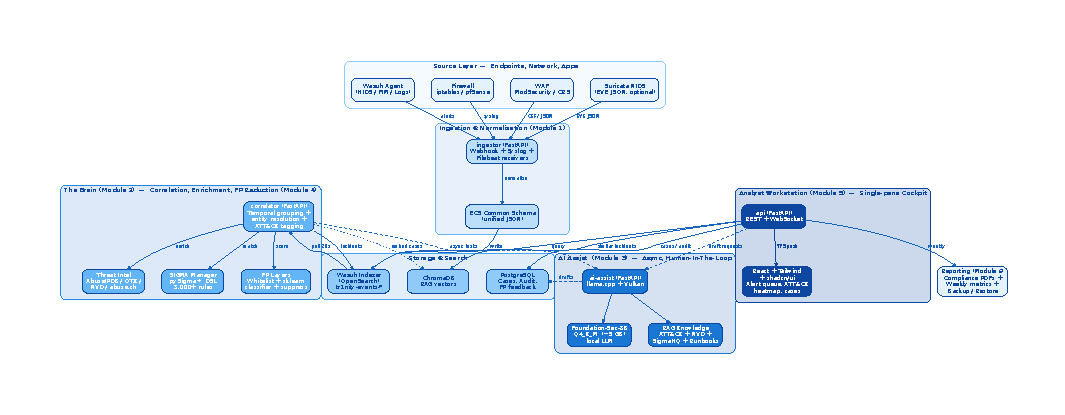
\includegraphics[width=0.95\linewidth, height=0.85\textheight, keepaspectratio]{figures/architecture.pdf}
  \caption{TR1NITY — Unified SIEM Correlation Platform Architecture. Six modules (Ingestion, The Brain, AI Assist, FP Handling, The Cockpit, Reporting) layered over Wazuh + firewall + WAF sources, with all data unified in a single OpenSearch index \texttt{tr1nity-events-*}.}
  \label{fig:arch}
\end{figure}
\end{landscape}

% ============== USE CASES ==============
\newpage
\section{Use Case Diagram + Description}
\label{sec:usecases}

\begin{figure}[H]
  \centering
  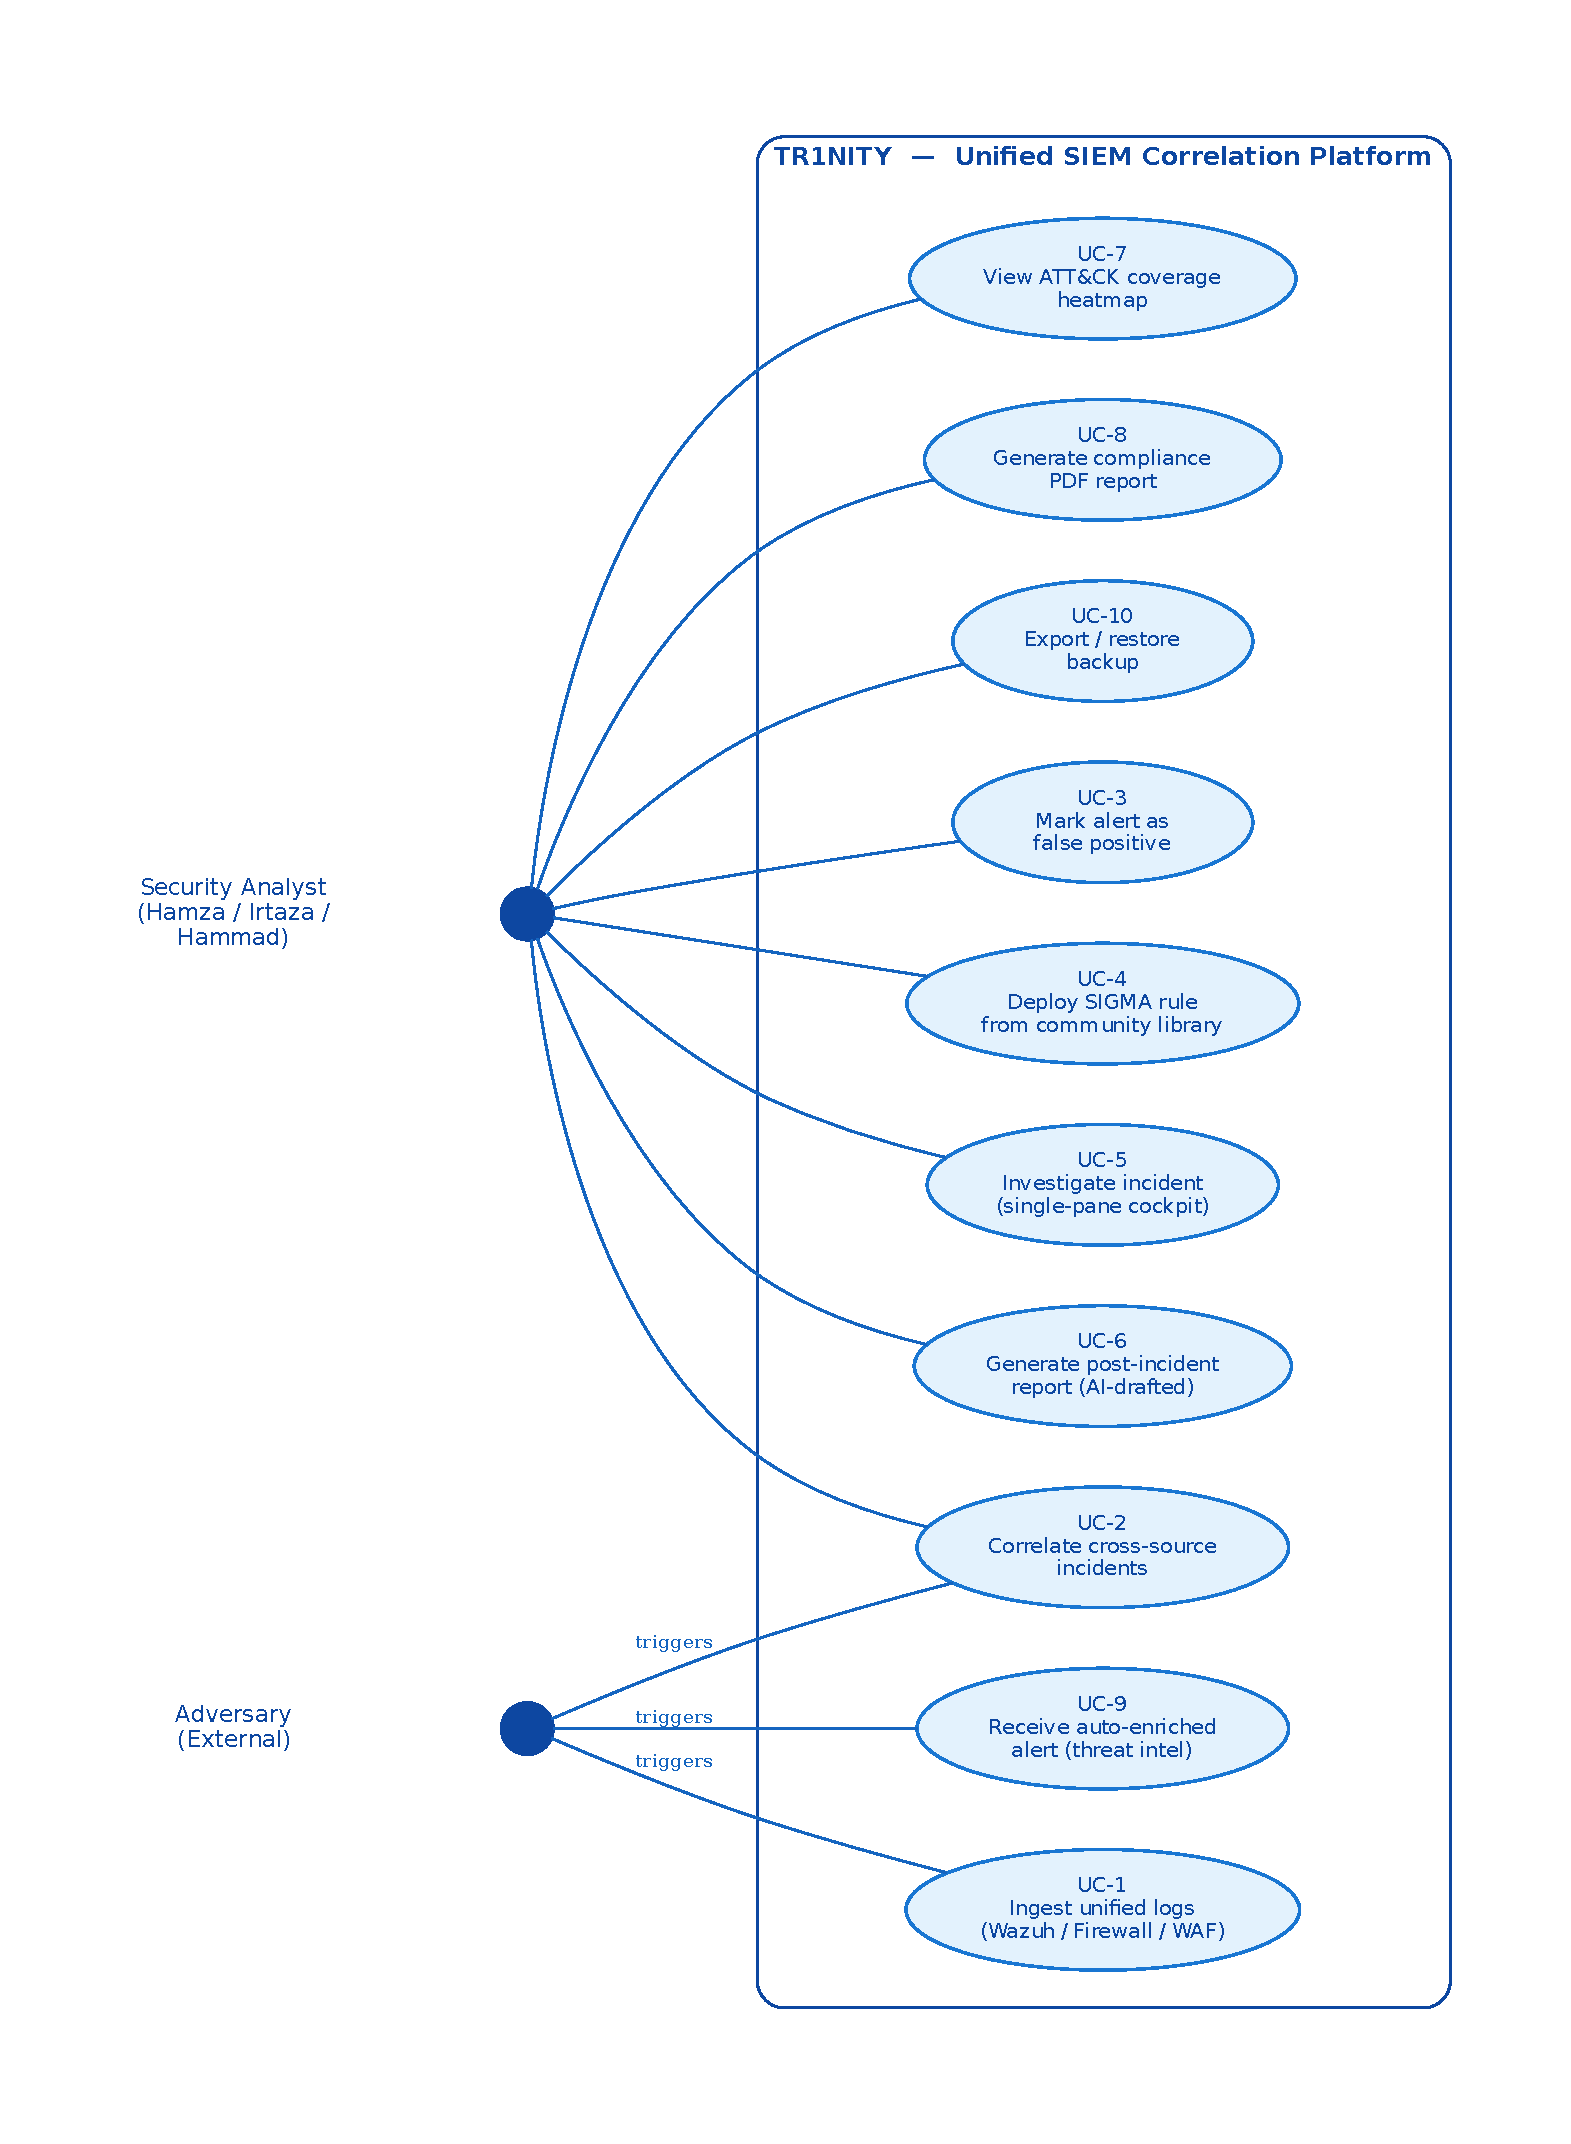
\includegraphics[width=0.95\textwidth]{figures/usecase.pdf}
  \caption{TR1NITY — Use Case Diagram. Primary actor: Security Analyst (Hamza, Irtaza, Hammad). Secondary actor: External Adversary.}
  \label{fig:usecase}
\end{figure}

\textbf{Use Case 1: Ingest Unified Wazuh + Firewall + WAF Logs.} \\
\textit{Actor:} Adversary (triggers), TR1NITY \texttt{ingestor} (system). \\
\textit{Precondition:} Wazuh agents installed, firewall syslog configured, ModSecurity audit log enabled. \\
\textit{Main Flow:} Attacker probes web app $\rightarrow$ ModSecurity blocks SQL-injection $\rightarrow$ firewall logs subsequent denied packets $\rightarrow$ Wazuh agent detects related FIM change $\rightarrow$ all three events arrive at \texttt{ingestor} $\rightarrow$ normalized to ECS $\rightarrow$ written to \texttt{tr1nity-events-*}. \\
\textit{Postcondition:} A single OpenSearch query for \texttt{source.ip:<attacker>} returns Wazuh, firewall, and WAF events sorted by time.

\textbf{Use Case 2: Correlate Cross-Source Incidents.} \\
\textit{Actor:} Adversary (triggers), \texttt{correlator} (system). \\
\textit{Precondition:} Events present in \texttt{tr1nity-events-*}. \\
\textit{Main Flow:} Adversary executes multi-stage attack chain $\rightarrow$ correlator's 30-second loop groups events by source IP within 5-minute window $\rightarrow$ resolves entities across Wazuh + firewall + WAF $\rightarrow$ tags MITRE ATT\&CK techniques $\rightarrow$ enriches with threat intel $\rightarrow$ writes single incident document. \\
\textit{Postcondition:} 5 raw events become 1 incident with full kill-chain and enrichment.

\textbf{Use Case 3: Mark Alert as False Positive.} \\
\textit{Actor:} Security Analyst. \\
\textit{Precondition:} Alert visible in queue. \\
\textit{Main Flow:} Analyst presses \texttt{f} (or clicks ``Mark FP'') $\rightarrow$ feature vector appended to SQLite feedback DB $\rightarrow$ confirmation toast. Weekly retrain ($\texttt{make retrain}$) re-fits the sklearn classifier and atomically swaps the pickle file. \\
\textit{Postcondition:} Future similar alerts receive a higher \texttt{fp\_score} and sort to the bottom of the queue.

\textbf{Use Case 4: Deploy SIGMA Rule from Community Library.} \\
\textit{Actor:} Security Analyst, Detection Engineer. \\
\textit{Precondition:} SigmaHQ submodule synced. \\
\textit{Main Flow:} Analyst browses 3,000+ rules in UI $\rightarrow$ selects rule $\rightarrow$ clicks ``Test'' (correlator runs the translated DSL against last 7 days, reports estimated FP rate) $\rightarrow$ if acceptable, clicks ``Deploy'' $\rightarrow$ rule activates in correlator. \\
\textit{Postcondition:} New detection live without restarting the platform.

\textbf{Use Case 5: Investigate Incident in Single-Pane Cockpit.} \\
\textit{Actor:} Security Analyst. \\
\textit{Precondition:} Incident in queue. \\
\textit{Main Flow:} Analyst presses \texttt{o} (open) $\rightarrow$ investigation panel renders raw payload (left), enrichment sidebar (right: AbuseIPDB + OTX + NVD + GeoIP + asset context), entity timeline (last 30 days for source IP / user / host), similar past incidents (semantic search via ChromaDB). \\
\textit{Postcondition:} Analyst makes verdict without opening any external tool.

\textbf{Use Case 6: Generate AI-Drafted Post-Incident Report.} \\
\textit{Actor:} Security Analyst, \texttt{ai-assist} service. \\
\textit{Precondition:} Case status set to ``resolved''. \\
\textit{Main Flow:} On case closure, \texttt{ai-assist} pulls all related events + analyst notes $\rightarrow$ retrieves grounding context from ChromaDB $\rightarrow$ Foundation-Sec-8B drafts a Markdown post-mortem $\rightarrow$ analyst reviews and edits in the Drafts queue $\rightarrow$ saves. \\
\textit{Postcondition:} Audit-grade incident report stored in PostgreSQL; both LLM output and analyst edits are preserved for future training.

\textbf{Use Case 7: View ATT\&CK Coverage Heatmap.} \\
\textit{Actor:} Security Analyst, Detection Engineer. \\
\textit{Precondition:} SIGMA rules deployed, recent events present. \\
\textit{Main Flow:} Analyst opens ATT\&CK Navigator panel $\rightarrow$ green = covered (deployed rule + recent test), yellow = covered but stale, red = uncovered $\rightarrow$ click cell to drill down to incidents under that technique. \\
\textit{Postcondition:} Detection-coverage gaps explicitly visible.

\textbf{Use Case 8: Generate Compliance PDF Report.} \\
\textit{Actor:} Security Analyst, Compliance Auditor. \\
\textit{Precondition:} 30+ days of operational data. \\
\textit{Main Flow:} User selects framework (PCI-DSS, ISO 27001, NIST CSF) and date range $\rightarrow$ \texttt{api} aggregates relevant alerts and control mappings $\rightarrow$ WeasyPrint renders PDF $\rightarrow$ download. \\
\textit{Postcondition:} Audit-ready compliance document delivered without analyst writing it.

\textbf{Use Case 9: Receive Auto-Enriched Alert with Threat Intel.} \\
\textit{Actor:} Security Analyst. \\
\textit{Precondition:} Threat-intel APIs reachable. \\
\textit{Main Flow:} New incident lands in queue with AbuseIPDB confidence score, OTX pulse matches, NVD CVE descriptions for any referenced vulnerabilities, GeoIP, ASN reputation — all already attached. \\
\textit{Postcondition:} Analyst makes triage decision in seconds, not minutes.

\textbf{Use Case 10: Export and Restore Backup.} \\
\textit{Actor:} Platform Administrator. \\
\textit{Precondition:} TR1NITY running. \\
\textit{Main Flow:} \texttt{make backup} tarballs feedback DB + cases + runbooks + ML models + SIGMA edits + suppressions + audit log. \texttt{make restore <file>} restores all of it on a clean install. \\
\textit{Postcondition:} Disaster-recovery story trivial; institutional knowledge portable.

% ============== TEST CASES ==============
\newpage
\section{Test Cases}
\label{sec:tests}

\begin{table}[H]
\small
\setlength{\tabcolsep}{4pt}
\begin{tabularx}{\textwidth}{|>{\columncolor{tr1BlueBg}}c|L{2.6cm}|L{3.4cm}|L{5.2cm}|c|}
\hline
\rowcolor{tr1Blue}\textcolor{white}{\textbf{TC ID}} & \textcolor{white}{\textbf{Description}} & \textcolor{white}{\textbf{Input}} & \textcolor{white}{\textbf{Expected Output}} & \textcolor{white}{\textbf{Status}} \\
\hline
TC-01 & Unified ingestion across Wazuh + Firewall + WAF & Synthetic event triplet (Wazuh FIM, iptables DROP, ModSecurity 403) for same source IP & Single OpenSearch query \texttt{source.ip:<x>} returns all 3 events; identical \texttt{event.module} field but unified ECS shape & Planned \\
\hline
TC-02 & Cross-source correlation & 5 events from 3 sources within 4 minutes for same IP & 1 incident document created with 5 event references; ATT\&CK techniques tagged & Planned \\
\hline
TC-03 & Brute force detection chain & 500 SSH failed logins from 1.2.3.4 in 5 min & Wazuh alert + firewall syslog correlated; AbuseIPDB enrichment attached; incident in queue with priority HIGH & Planned \\
\hline
TC-04 & SIGMA rule deploy + test & Selection of SigmaHQ rule \texttt{T1110.001} & pySigma translates to OpenSearch DSL; test run against last 7 days returns FP estimate; rule deployable & Planned \\
\hline
TC-05 & False-positive feedback loop & Analyst marks 50 alerts as FP; \texttt{make retrain} & New sklearn pickle deployed atomically; held-out sample shows reduced FP score on similar alerts & Planned \\
\hline
TC-06 & Threat-intel enrichment with caching & 1,500 incidents in one day referencing 80 unique IPs & AbuseIPDB call count $<$ 100 (24-hour cache hit rate $>$ 90\%); free tier preserved & Planned \\
\hline
TC-07 & Single-pane investigation & Open random incident in UI & Raw payload, enrichment sidebar, entity timeline, similar incidents all render; no second tool required & Planned \\
\hline
TC-08 & AI-drafted post-incident report & Close a case via UI & Foundation-Sec-8B Q4 (Vulkan) drafts markdown report in $<$30 s; analyst sees ``Draft ready'' badge & Planned \\
\hline
TC-09 & Mock LLM mode & Set \texttt{MOCK\_LLM=true} and rerun TC-08 & Deterministic templated report returned; no GPU/CPU LLM invoked; UI flow identical & Planned \\
\hline
TC-10 & ATT\&CK heatmap accuracy & Run synthetic attack chain spanning T1046 + T1110 + T1078 + T1041 & Heatmap shows green for the 4 techniques; click drills down to the originating incident & Planned \\
\hline
TC-11 & Compliance PDF generation & Generate PCI-DSS report for last 30 days & PDF rendered with audit-trail evidence per control; valid section numbering; download link in UI & Planned \\
\hline
TC-12 & Backup / Restore round trip & \texttt{make backup} on populated install; \texttt{make restore} on clean install & Cases, FP labels, runbooks, ML models, SIGMA edits identical post-restore & Planned \\
\hline
\end{tabularx}
\caption{TR1NITY Phase-1 planned test cases, mapped to the six modules.}
\end{table}

% ============== MARKET VALUE ==============
\newpage
\section{Market Value}
\label{sec:market}

\subsection{Target Users}
TR1NITY directly targets four user classes:

\begin{itemize}[leftmargin=*, itemsep=2pt]
  \item \textbf{Small and medium-sized businesses (SMBs)} that cannot afford commercial SIEM/SOAR licensing ($\$30{,}000$--$\$500{,}000$/year for Splunk, IBM QRadar, Microsoft Sentinel) but operate enough infrastructure to need real correlation across host, perimeter, and web layers.
  \item \textbf{University cybersecurity programs and SOC labs} that need realistic, teachable, fully-open SOC pipelines. TR1NITY's runbooks, synthetic attack chain, and explicit free-tier API design make it directly usable as course material.
  \item \textbf{Junior SOC analysts and detection engineers} learning blue-team tradecraft. The single-pane cockpit and 15+ runbooks compress the typical 6-month onboarding cliff.
  \item \textbf{Managed Security Service Providers (MSSPs)} serving cost-sensitive clients. The open-source license, free-only API design, and Docker-Compose deployment enable per-client instance deployment without licensing overhead. (Multi-tenant operation is a v2.0 roadmap item.)
\end{itemize}

\subsection{Market Relevance}
The global SIEM market was valued at approximately $\$5.2$ billion in 2024 and is projected to grow at a 14\% CAGR through 2029, driven by regulatory pressure and rising attack volume. Concurrently, surveys consistently indicate that 71\% of SOC analysts report some level of burnout and 64\% intend to leave their role within a year, primarily due to alert fatigue \cite{secure2024burnout}. The mismatch is acute: the market is growing faster than the analyst pool, and existing options polarize between expensive commercial suites (Splunk, QRadar, Sentinel) and disconnected free tools that still require heavy manual stitching. TR1NITY occupies the missing ``unified open-source'' position with an AI-assisted differentiator that aligns with empirical analyst preferences (async drafting, not real-time triage) \cite{darrow2024aisoc}.

\subsection{Economic Positioning}
\textbf{Net recurring cost: \$0.} Every external dependency is verified free-tier. AbuseIPDB free (1,000 IP checks/day, 100 block checks/day, no credit card), AlienVault OTX (free), NVD CVE API v2 (free with optional API key), abuse.ch (MalwareBazaar, URLhaus, ThreatFox; free), MaxMind GeoLite2 (free monthly auto-update), MITRE ATT\&CK STIX 2.1 (free), SigmaHQ rules (free, MIT/DRL), Foundation-Sec-8B (Apache 2.0), Wazuh (GPLv2), Wazuh Indexer / OpenSearch (Apache 2.0), Filebeat OSS (Apache 2.0), GitHub Actions (free for public repos), GitHub Container Registry (unlimited free for public images). The only ``cost'' to the user is the electricity to run the host and (optionally) a one-time GPU upgrade if the existing GPU lacks Vulkan support.

\subsection{Competitor Comparison}

\begin{table}[H]
\small
\setlength{\tabcolsep}{6pt}
\begin{tabularx}{\textwidth}{|>{\columncolor{tr1BlueBg}}L{2.8cm}|L{2.4cm}|L{3.0cm}|L{2.4cm}|L{3.4cm}|}
\hline
\rowcolor{tr1Blue}\textcolor{white}{\textbf{Product}} & \textcolor{white}{\textbf{Type}} & \textcolor{white}{\textbf{AI Integration}} & \textcolor{white}{\textbf{Price}} & \textcolor{white}{\textbf{Unified Wazuh+FW+WAF}} \\
\hline
Splunk Enterprise Security & Commercial & Limited (Splunk AI Assistant, paid) & \$50{,}000+/year & Possible via custom apps; not built-in \\
\hline
IBM QRadar SIEM & Commercial & Yes (Watson, paid) & \$30{,}000+/year & Partial (firewall + Wazuh-equivalent) \\
\hline
Microsoft Sentinel & Commercial & Yes (Security Copilot, usage-based) & Usage-based, $\$2$+/GB ingest & Partial (Defender ecosystem) \\
\hline
Elastic Security & Freemium & Paid LLM features in Platinum tier & Free OSS / paid Platinum & DIY integration; no analyst UI \\
\hline
Wazuh standalone & Open Source & None & Free & No (Wazuh-only) \\
\hline
\rowcolor{tr1BlueBg}TR1NITY & Open Source (MIT) & Local Foundation-Sec-8B (Apache 2.0); HITL only & Free & \textbf{Yes — first of its kind in OSS} \\
\hline
\end{tabularx}
\caption{TR1NITY positioning vs. dominant SIEM/SOC platforms.}
\end{table}

% ============== GANTT CHART ==============
\newpage
\section{Gantt Chart}
\label{sec:gantt}

\begin{figure}[H]
  \centering
  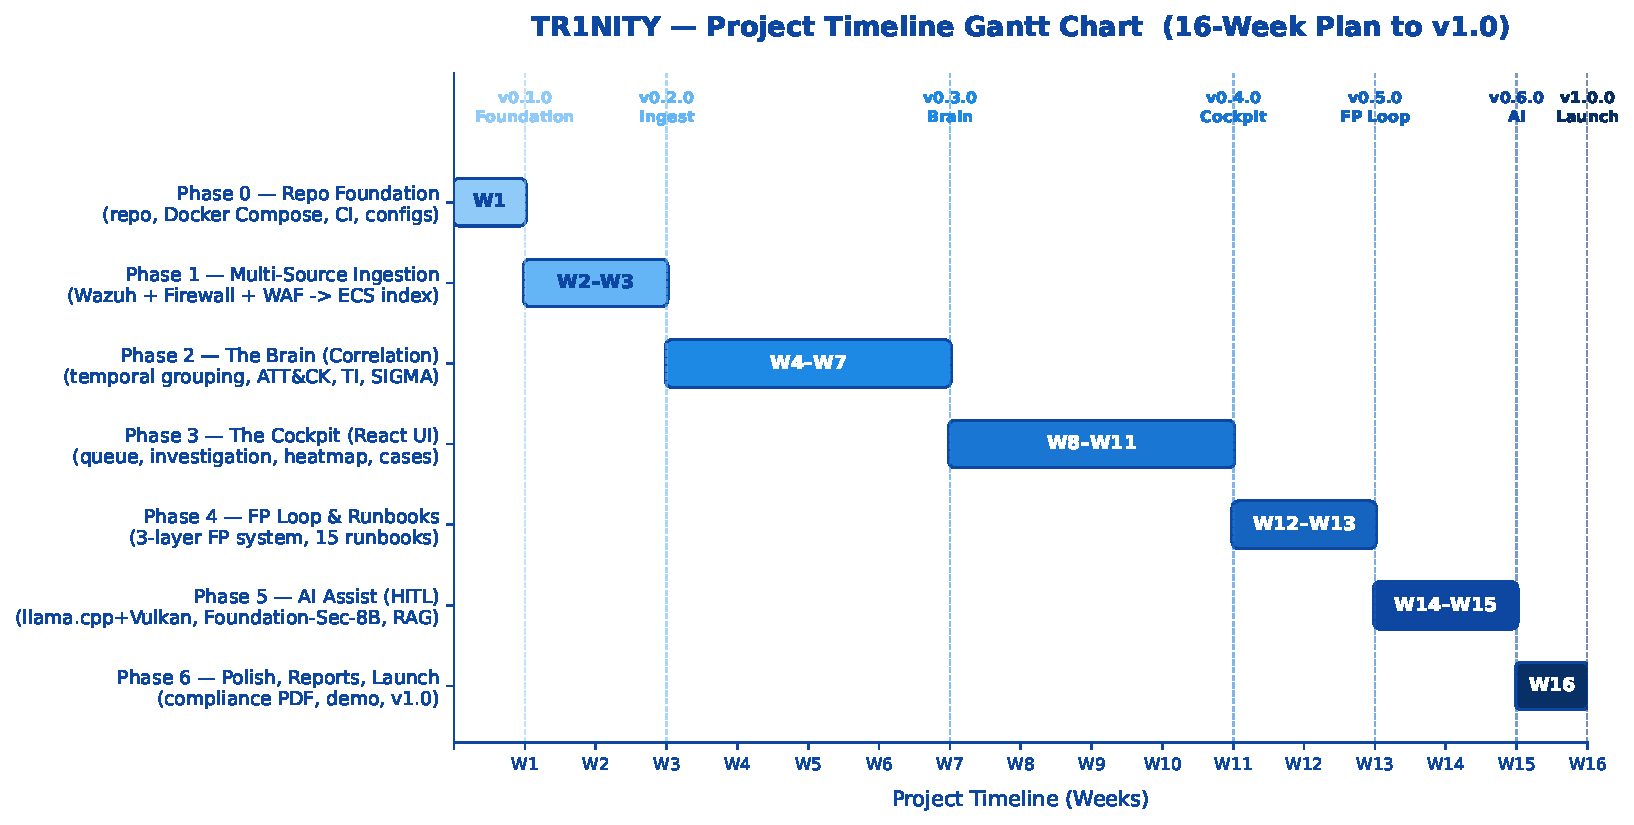
\includegraphics[width=\textwidth]{figures/gantt.pdf}
  \caption{TR1NITY — Project timeline (16-week plan to v1.0). Each phase ends with a tagged release and a demoable \texttt{make} command so progress is always visible.}
  \label{fig:gantt}
\end{figure}

The TR1NITY implementation plan is structured into seven phases:

\begin{enumerate}[leftmargin=*, itemsep=2pt]
  \item \textbf{Phase 0 — Repository Foundation (Week 1).} Repo creation, MIT license, Docker Compose skeleton (Wazuh + indexer + dashboard + 4 service hello-worlds), GitHub Actions CI, MkDocs site, configuration system. \textit{Tag: v0.1.0-foundation}.
  \item \textbf{Phase 1 — Multi-Source Ingestion (Weeks 2--3).} Wazuh integration, firewall syslog parser, ModSecurity ingestion, ECS schema, ISM index lifecycle policy. \textit{Tag: v0.2.0-ingest}.
  \item \textbf{Phase 2 — The Brain (Weeks 4--7).} Correlation engine, entity resolution, ATT\&CK tagging, threat-intel enrichment, SIGMA rule import + deploy + test, runbook auto-attach. \textit{Tag: v0.3.0-brain}.
  \item \textbf{Phase 3 — The Cockpit (Weeks 8--11).} React + Tailwind + shadcn UI; alert queue, single-pane investigation panel, ATT\&CK heatmap, similar-incidents search, lightweight case manager, audit trail. \textit{Tag: v0.4.0-cockpit}.
  \item \textbf{Phase 4 — FP Loop \& Runbooks (Weeks 12--13).} 3-layer FP system (whitelist + sklearn classifier + suppression rules); 15+ markdown runbooks; per-alert auto-attach by ATT\&CK technique. \textit{Tag: v0.5.0-feedback}.
  \item \textbf{Phase 5 — AI Assist (Weeks 14--15).} \texttt{llama.cpp} build with Vulkan backend; Foundation-Sec-8B Q4 deployment; ChromaDB ingest; async drafting endpoints (incident report, runbook, CVE explanation); MOCK\_LLM mode. \textit{Tag: v0.6.0-ai}.
  \item \textbf{Phase 6 — Polish, Reporting, Launch (Week 16).} Compliance PDF generator (PCI-DSS, ISO 27001, NIST CSF), weekly metrics report, backup/restore, README polish with demo GIF, demo video, public launch. \textit{Tag: v1.0.0}.
\end{enumerate}

The schedule is aligned to a hard completion deadline of \textbf{16 weeks} from project kickoff, with each phase ending in a tagged release and a demoable \texttt{make} command. Cadence is enforced over perfection: the project never spends more than 4 weeks without producing a visible deliverable.

% ============== RESULTS & CONCLUSION ==============
\newpage
\section{Results \& Conclusion}
\label{sec:results}

\subsection{Expected Outcomes}

\begin{itemize}[leftmargin=*, itemsep=3pt]
  \item \textbf{Unified ingestion across three log sources} (Wazuh, firewall, WAF) into a single OpenSearch index with one ECS-compatible schema, queryable through one interface.
  \item \textbf{Real-time cross-source correlation:} multi-stage attack chains spanning host, perimeter, and web layers reduced to a single incident document with full kill-chain.
  \item \textbf{False-positive rate below 30\%} of unfiltered Wazuh+firewall+WAF output within two weeks of analyst feedback (3-layer FP pipeline).
  \item \textbf{Threat intelligence auto-enrichment} on every incident (AbuseIPDB, AlienVault OTX, NVD, abuse.ch, MaxMind GeoLite2) — all from free APIs, with caching to remain within free-tier limits.
  \item \textbf{Single-pane investigation:} 80\% of alerts fully triaged without opening a second tool.
  \item \textbf{AI-drafted post-incident reports} generated locally by Foundation-Sec-8B Q4 via \texttt{llama.cpp}+Vulkan on RX 590; analyst reviews and edits before saving.
  \item \textbf{ATT\&CK coverage heatmap} showing detection gaps; SigmaHQ community rules ($>$2{,}000) deployable in one click.
  \item \textbf{Compliance reporting} (PCI-DSS, ISO 27001, NIST CSF) auto-generated as PDF.
  \item \textbf{Quickstart from \texttt{git clone} to first alert in under 15 minutes} on a 16~GB host.
  \item \textbf{Estimated 70\% reduction in time-to-triage} for alerts that historically required cross-tool stitching.
\end{itemize}

\subsection{Summary of Planning Phase}

Phase 1 has formalized TR1NITY's strategic and technical foundation. The documentation defined the precise SOC pain point — fragmented Wazuh + firewall + WAF tooling combined with crippling alert fatigue — and mapped a six-module architecture with explicit, evidence-grounded design decisions: a unified ECS schema for all three log sources; a deterministic correlation core; a free-only threat-intel layer; a 3-layer false-positive pipeline learning from analyst feedback; a single-pane analyst UI built with production-grade React tooling; and a deliberately-scoped, asynchronous, human-in-the-loop AI assistant aligned with empirical findings on AI in real SOCs \cite{darrow2024aisoc}.

The phase produced a complete integration blueprint with selected technologies (all free and open-source), core workflows, ten use cases, twelve test cases, a sixteen-week execution timeline with seven tagged releases, and a market positioning grounded in the genuine cost-coverage gap left by commercial SIEMs. As a result, TR1NITY transitions into implementation with defined interfaces, expected outputs, validation criteria, and a clear adoption story. This creates a low-risk path to delivering the first widely-adoptable open-source platform that unifies Wazuh, firewall, and WAF correlation under a locally-hosted AI assistance layer with zero recurring cost.

% ============== REFERENCES ==============
\newpage
\section{References}
\label{sec:refs}
\printbibliography[heading=none]

% ============== APPENDIX ==============
\newpage
\section{Appendix}
\label{sec:appendix}

\subsection{Appendix A: Module Listing (Detailed)}

\begin{longtable}{|>{\columncolor{tr1BlueBg}}L{2.4cm}|L{4.6cm}|L{3.0cm}|L{4.5cm}|}
\hline
\rowcolor{tr1Blue}\textcolor{white}{\textbf{Module}} & \textcolor{white}{\textbf{Responsibilities}} & \textcolor{white}{\textbf{Tech Stack}} & \textcolor{white}{\textbf{Phase / Tag}} \\
\hline
\endhead
M1 — Ingestion \& Normalization & Receive Wazuh webhooks, firewall syslog, ModSecurity logs, optional Suricata EVE; map all to ECS schema; write to \texttt{tr1nity-events-*}. & FastAPI, Pydantic, Filebeat, asyncio syslog server & Phase 1 (W2--3) \newline v0.2.0-ingest \\
\hline
M2 — Correlation \& Enrichment (The Brain) & Temporal grouping, entity resolution, ATT\&CK tagging, threat-intel enrichment with caching, SIGMA rule import / deploy / test, runbook attachment. & FastAPI, pySigma, scikit-learn, requests, Redis or LRU cache & Phase 2 (W4--7) \newline v0.3.0-brain \\
\hline
M3 — AI Assist (HITL) & Async drafting of incident reports, runbooks, compliance summaries, CVE explanations. Local LLM with Vulkan acceleration on RX 590. RAG-grounded. & FastAPI, llama.cpp + Vulkan, Foundation-Sec-8B-Instruct Q4\_K\_M, ChromaDB & Phase 5 (W14--15) \newline v0.6.0-ai \\
\hline
M4 — False-Positive Handling & 3 layers: deterministic YAML whitelists; sklearn classifier learning from analyst feedback; analyst-authored suppression rules. Weekly retrain via \texttt{make retrain}. & sklearn (RandomForest), SQLite, YAML, cron & Phase 4 (W12--13) \newline v0.5.0-feedback \\
\hline
M5 — Analyst Workstation (The Cockpit) & Alert queue, single-pane investigation panel, ATT\&CK heatmap, similar-incidents search, lightweight case management, audit trail, keyboard shortcuts. & React, TypeScript, Tailwind, shadcn/ui, TanStack Query, ChromaDB, FastAPI WebSocket & Phase 3 (W8--11) \newline v0.4.0-cockpit \\
\hline
M6 — Knowledge, Audit \& Reporting & 15+ runbooks, audit trail, compliance PDFs (PCI-DSS, ISO 27001, NIST CSF), weekly metrics report, backup/restore. & WeasyPrint / ReportLab, PostgreSQL, cron, Markdown & Phase 6 (W16) \newline v1.0.0 \\
\hline
\end{longtable}

\subsection{Appendix B: Tool / API Summary Table (Free-Tier Verified)}

\begin{longtable}{|>{\columncolor{tr1BlueBg}}L{2.4cm}|L{2.0cm}|L{3.6cm}|L{2.6cm}|L{3.0cm}|}
\hline
\rowcolor{tr1Blue}\textcolor{white}{\textbf{Tool / Service}} & \textcolor{white}{\textbf{API Type}} & \textcolor{white}{\textbf{Endpoint / Mode}} & \textcolor{white}{\textbf{Auth}} & \textcolor{white}{\textbf{Free Tier Limit}} \\
\hline
\endhead
Wazuh Manager & REST/JSON & \texttt{/security/events} & API token & Configurable (self-hosted) \\
\hline
Wazuh Indexer (OpenSearch) & REST/JSON & \texttt{/index/\_search} & Basic / API key & Cluster policy (self-hosted) \\
\hline
Filebeat & TCP / Log file & Forwarder to ingestor & TLS optional & N/A (local) \\
\hline
ModSecurity (CRS) & Audit log / syslog & JSON or CEF format & N/A (local) & N/A (local) \\
\hline
Suricata (optional) & EVE JSON local stream & Local socket / file & N/A (local) & N/A (sensor-bound) \\
\hline
AbuseIPDB & REST & \texttt{/api/v2/check} & API key & 1{,}000 checks + 100 block checks/day; free forever; no CC \\
\hline
AlienVault OTX & REST & \path{/api/v1/indicators/} & API key & Free; rate-limited per minute \\
\hline
NVD CVE API v2 & REST & \texttt{/rest/json/cves/2.0} & Optional API key & 50 req / 30 s (with key); 5 req / 30 s without \\
\hline
abuse.ch (MalwareBazaar / URLhaus / ThreatFox) & REST & Public APIs & None (or free auth-key) & Free; reasonable use \\
\hline
MaxMind GeoLite2 & DB download & Monthly DB pull & License key (free) & Free; one DB pull/day \\
\hline
MITRE ATT\&CK STIX 2.1 & Static JSON & \path{github.com/mitre-attack/attack-stix-data} & None & Free; quarterly updates \\
\hline
SigmaHQ & Static rules repo & \path{github.com/SigmaHQ/sigma} & None & Free (MIT/DRL); $\sim$3{,}000 rules \\
\hline
Foundation-Sec-8B-Instruct Q4\_K\_M & Local model & GGUF via llama.cpp & N/A (local) & Free (Apache 2.0); $\sim$5\,GB \\
\hline
ChromaDB & In-process Python lib & \texttt{from chromadb import Client} & N/A & Free (Apache 2.0) \\
\hline
TR1NITY ingestor / correlator / ai-assist / api & REST + WebSocket & FastAPI services & API key / JWT (self-hosted) & Free (MIT — TR1NITY) \\
\hline
GitHub Actions CI & Hosted CI & GitHub-hosted runners & GitHub token & 2{,}000 minutes/month (free tier) \\
\hline
GitHub Container Registry & OCI registry & \path{ghcr.io/<user>/tr1nity-*} & GitHub token & Unlimited free for public images \\
\hline
\end{longtable}

\subsection{Appendix C: System Requirements}

\noindent\textbf{Recommended Hardware (production / demo):}
\begin{itemize}[leftmargin=*, itemsep=2pt]
  \item CPU: 8-core x86\_64 (AMD Ryzen 7 3700X or equivalent / Intel i7 12th gen+)
  \item RAM: 16~GB DDR4 (32~GB recommended for full AI mode + heavier indices)
  \item GPU (optional but recommended for AI Assist): AMD RX~590 (8~GB VRAM, Vulkan) or NVIDIA equivalent (CUDA). CPU fallback supported via \texttt{llama.cpp}.
  \item Storage: 500~GB SSD (1~TB for $>$90-day index retention)
  \item Network: standard LAN; mirror/SPAN port optional (Suricata)
\end{itemize}

\noindent\textbf{Minimum Hardware (Standard profile):}
\begin{itemize}[leftmargin=*, itemsep=2pt]
  \item CPU: 4-core x86\_64
  \item RAM: 8~GB (LLM disabled; \texttt{MOCK\_LLM=true})
  \item Storage: 100~GB SSD
\end{itemize}

\noindent\textbf{Software Requirements:}
\begin{itemize}[leftmargin=*, itemsep=2pt]
  \item OS: Ubuntu 22.04 LTS (primary), Debian 12, or Fedora 40+ (host or VM)
  \item Container Runtime: Docker Engine 24+ \& Docker Compose plugin v2.20+
  \item Core Stack (auto-pulled by \texttt{docker compose up}): Wazuh manager + indexer + dashboard, PostgreSQL, TR1NITY services
  \item LLM Runtime: \texttt{llama.cpp} built with \texttt{-DGGML\_VULKAN=ON} (or CPU-only)
  \item Python: 3.11+ (for any out-of-container scripts)
  \item Languages / Toolchains for development: Python 3.11, Node.js 20+, npm or pnpm
\end{itemize}

\noindent\textbf{Required External Accounts (all free, none paid):}
\begin{itemize}[leftmargin=*, itemsep=2pt]
  \item AbuseIPDB account (free forever)
  \item AlienVault OTX account (free)
  \item NVD CVE API key (free, optional, raises rate limit)
  \item MaxMind GeoLite2 license key (free, monthly DB)
  \item GitHub account (for cloning, CI, container registry)
\end{itemize}

\noindent\textbf{GitHub Repository Storage Strategy:}
\begin{itemize}[leftmargin=*, itemsep=2pt]
  \item Source code, configs, runbook markdowns, Docker Compose YAML — \textbf{in-repo} ($\sim$50~MB total).
  \item MITRE ATT\&CK STIX, SigmaHQ rules — \textbf{git submodules} ($\sim$55~MB combined).
  \item Trained ML models — \textbf{GitHub Releases assets} (up to 2~GB per asset, unlimited storage, free).
  \item Docker images — \textbf{GitHub Container Registry} (unlimited free for public images).
  \item Datasets (CICIDS2017 8~GB, UNSW-NB15 2~GB) — \textbf{not redistributed}; pulled by the helper script \texttt{download\_datasets.sh} (under \texttt{scripts/}) from official mirrors.
  \item LLM weights — \textbf{not redistributed}; pulled via \texttt{ollama pull} or \texttt{huggingface-cli download}.
  \item Pre-commit hook rejects any single file $>$10~MB. Final repo size at v1.0: $<$100~MB.
\end{itemize}

\end{document}
